\documentclass[11pt]{article}
\usepackage{amsmath}
\usepackage{geometry}                % See geometry.pdf to learn the layout options. There are lots.
\geometry{letterpaper}                   % ... or a4paper or a5paper or ... 
%\geometry{landscape}                % Activate for for rotated page geometry
%\usepackage[parfill]{parskip}    % Activate to begin paragraphs with an empty line rather than an indent
\usepackage{graphicx}
\usepackage{amssymb}
\usepackage{epstopdf}
\DeclareGraphicsRule{.tif}{png}{.png}{`convert #1 `dirname #1`/`basename #1 .tif`.png}

%Don't list section numbers
\setcounter{secnumdepth}{0}

\title{CS 1653: Applied Cryptography and Network Security\\Term Project, Phase 4}
\author{Lindsey ``Hellman" Bieda\quad\texttt{leb35@pitt.edu}\\Tucker ``Diffie" Trainor\quad\texttt{tmt33@pitt.edu}}
\date{April 5, 2012} % Activate to display a given date or no date

\begin{document}
\maketitle
\section{Introduction: Cryptographic Techniques}
The additional threats to our Secure File Server model present new challenges to ensuring the confidentiality and integrity of a user's data. To protect against these threats, we can introduce cryptographic techniques that either augment or supplement existing methods that addressed Threats 1-4.

We will continue to use AES for symmetric key encryption, and to ensure against tampering of AES encrypted messages we will employ HMAC with SHA1 to authenticate messages sent over an encrypted channel. Embedding sequence numbers into messages will also help in detecting replay or reordering by a malicious agent. To combat against file leakage and maintain group privileges over file access, files saved on any File Server will be encrypted with AES, the keys of which will be created and maintained by the Group Server, which will generate them with a reasonably secure pseudorandom number generator and strictly control how they are released to authorized group members. 
% Threat 5
\section{Threat 5: Message Reorder, Replay, or Modification}
\subsection{Threat Description}
Whereas Threats 1-4 encompassed the possible efforts of a \emph{passive} attacker that could only eavesdrop on connections between clients and servers, Threat 5 now introduces the danger of an \emph{active} attacker who is capable of inserting, reordering, replaying, or modifying messages. Though encryption of the communication channel was enough to thwart a passive attacker and maintain confidentiality, an active attacker is able to disrupt the integrity of communications by effectively nullifying messages by tampering with them.

Reordering and replaying of messages can convince either end of a communication channel that the other party wishes to perform an action that is not what is actually intended by that party despite the correctness of the mechanism. An active attacker can also alter the message itself at the bit level, causing changes that could randomly alter the intention of the message or garble it completely. Modification is not only an affront to the integrity of the Secure File Server model but also can reduce availability if no message can be trusted as to its accuracy.
\subsection{Mechanism Description}
The mechanism builds upon the protocols used in Threats 1-4 that establish a secure session key between a client and a server. Though messages passed in the session are secure from eavesdropping, they are not secure from reorder, replay, or modification. We use two methods to eliminate these new threats: sequence numbers and message authentication.
\begin{figure}[htbp]
\begin{center}
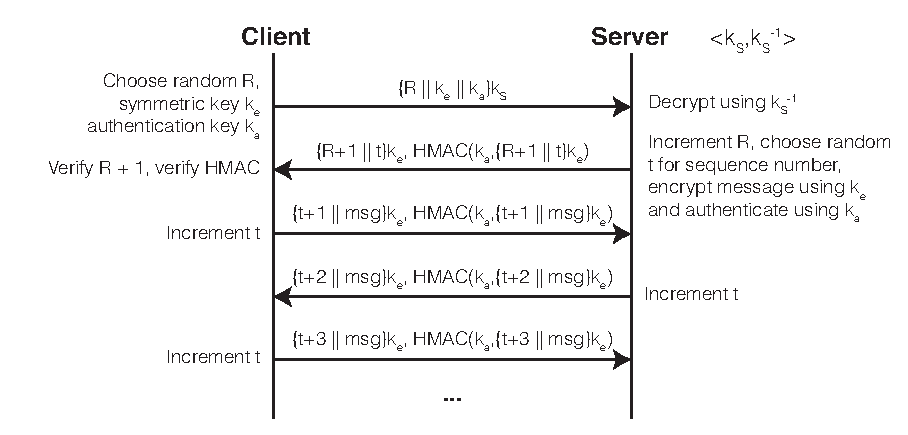
\includegraphics{threat5.eps}
\caption{Threat 5 Mechanism}
\label{threat5}
\end{center}
\end{figure}

Sequence numbers are a simple yet effective tool that would alert either end of channel that a message has ben reordered or replayed. We modify our message format so that it includes an integer field to store the sequence number. Then, after receiving a message, the receiving party increments the sequence number by 1 and uses that value in their response. Replays and reordering of messages are easily detectable by either party, as the sequence number will reveal an inconsistency. To prevent a replay of the entire session, we restrict the initiator of the session (i.e., the Client) to choosing the challenge \textsf{R}, and the responder (i.e., the Server) to choosing the random sequence number \textsf{t}.

Message authentication is a cryptographic principal that is used to verify that a message has not been tampered with. We have chosen the HMAC with SHA1 protocol to authenticate messages. To use HMAC in the most secure manner, we need to create an additional shared secret key to use for the keyed hash of HMAC. We can do this at the same time as the creation of the shared secret key for the AES symmetric encryption. With these two keys, \textsf{k}$_\textsf{e}$ for encryption and \textsf{k}$_\textsf{a}$ for authentication, we can create an authentication mechanism that addresses Threat 5. The sequence number and message are encrypted with \textsf{k}$_\textsf{e}$, and then the HMAC is done using \textsf{k}$_\textsf{a}$ on the encrypted sequence number and message (see Figure \ref{threat5}). The receiver of the encrypted message and HMAC digest will then be able to verify against tampering.
\subsection{Correctness and Security of Mechanism}
The correctness of the mechanism is similar to that of Threat 4: Information Leakage via Passive Monitoring. The creation of the challenge and checking the response is crucial if the Client is to verify that the responding Server is who they claim to be, which is proven by successful decryption of the challenge using the Server's private key. The addition of a sequence number to the mechanism means that both parties must keep track of the incrementation of the number to ensure that replay has not occurred--if either party finds that the number has not been properly incremented (e.g., a \textsf{t} value of 57 is sent, but a \textsf{t} value of 59 is returned) then the party must terminate the session. Both parties must also be responsible for using the encryption and authentication keys correctly and consistently for every message exchange.

The security of the mechanism is ensured by the message authentication protocols and the sequence numbering. Any modification to a message will be evident when the receiver uses HMAC with shared authentication key to verify the message. If the digest values do not agree, then tampering has been detected and the receiver should terminate the session. Sequence numbers provide security against replay and reordering. With both parties of a session keeping track of a sequence number, a replay of any previous message is easily detectable by the receiver, as the sequence number will be less than what is expected by the receiver. By requiring the Client to choose \textsf{R} and the Server to choose \textsf{t}, we can also detect replay of an entire session as each side of the exchange is choosing a random number at the outset of the session, and thus the probability of a replay successfully containing the correct responses to challenges or sequence initiation is insignificant. Reordering of messages is also easily detectable when each party is checking sequence numbers, as any message that does not contain the expected sequence number is suspect.
% Threat 6
\section{Threat 6: File Leakage}
\subsection{Threat Description}
The threat of file leakage represents a major vulnerability of the previous set of threats to our model. Previously, files saved to a File Server were encrypted over the network but not in storage. Therefore, an untrusted File Server could leak fully readable files that any user, malicious or not, could read. Obviously, we must encrypt the files to protect them against unauthorized access, but at the same time we must also enforce group privileges where only group members have access to the files and also maintain security by preventing former group members from accessing files created after their dismissal.
\subsection{Mechanism Description}
If groups were limited to just their owners, the threat could easily be eliminated with a single secret key for all files that was only known by or accessible to the owner. However, the fluid nature of groups quickly complicates this ideal and requires a more elaborate mechanism.

Because of how group membership is tied to file access, we use the Group Server to generate and store symmetric secret keys for group files. The Group Server maintains a \texttt{Hashtable} object with \texttt{<K,V>} parameters \texttt{<String groupName, ArrayList<Key> keyList>}. Upon creation of a new group, the Group Server creates a random 128-bit AES key that is stored under the group's name in the hash table. As additional keys for a group are needed, they are randomly generated and added to that group's \texttt{ArrayList}.
\begin{figure}[htbp]
\begin{center}
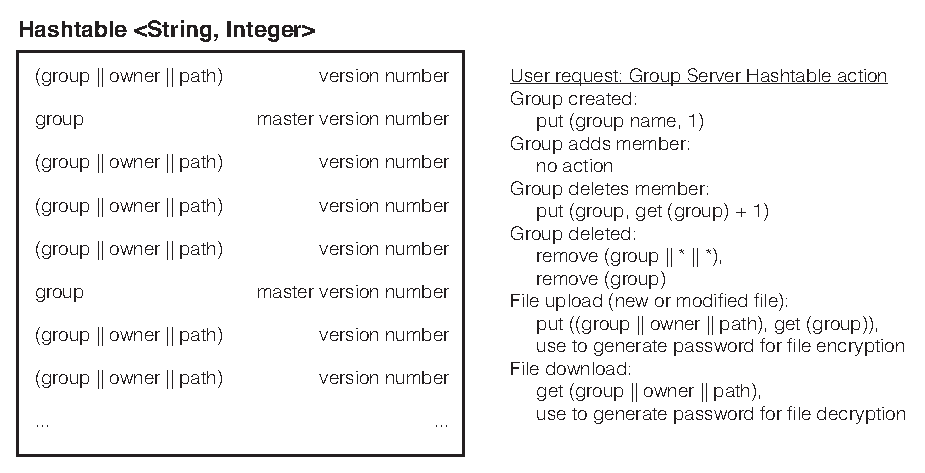
\includegraphics{threat6.eps}
\caption{Threat 6 Mechanism}
\label{threat6}
\end{center}
\end{figure}

For group members to access a set of keys for use in the File Client, they must authenticate themselves to the Group Server via username/password authentication. An authenticated group member will then submit to the Group Server the group which they wish to upload or download to. The Group Server embeds the keys for that particular group in the group member's token and returns it to the group member. The group member may now use the File Client to encrypt and upload files or download and decrypt files.

Though the File Server should never see any group keys, it must be aware of which key was used to encrypt the file which is has stored. We modify the \textsf{ShareFile} class to include the key version, which is simply the index of the key in the \textsf{ArrayList} where the group's keys are stored. When a file is uploaded to the File Server, the most recent key (i.e., the key with the highest index number) is used to encrypt the file. The user uploading the file will send the key version (index number) to the File Server as part of the upload process. When the File Server receives a request to download a file, it will include the key version with the encrypted file so that the File Client can use the correct key from the user's token to decrypt the file.
\subsection{Correctness and Security of Mechanism}
The correctness of the mechanism relies on proper distribution of keys and accurate record keeping of files and the key versions used to encrypt them. The onus of distribution falls on the Group Server, which must authenticate a user, check that the user is in fact a member of a particular group, and finally provide the user with a token that contains the keys the user will need to successfully interact with the File Server through the File Client. The record keeping of files and key versions is handled by the File Server through its \textsf{ShareFile} class. For the File Server to do its part, it must be given the key version by the user through the File Client. Without the key version number, the File Client would be unable to decrypt file as it would not know which key to use.

To illustrate the security of the mechanism, we need to fully explain the handling of key version numbers and how it affects forward and backward secrecy as group membership changes. The primary event that creates a new key is when a member is removed from a group. When that occurs, a new key is created by the Group Server and this new key will be used by existing group members to encrypt uploaded files. Let us call the set of keys before the group change $V$, and the set of keys after the group change $V^\prime$.

If the expelled group member was generally unmalicious, then when he or she tries to access files from their former group, the Group Server would see that the user was no longer in the group and deny access to the group's key set. Any previous downloads of unencrypted group files cannot be prevented, but future attempts at downloads by a user playing by the rules are thwarted. If the user was more malicious, he or she may have been able to, while still a group member, extract the key set $V$ from their token. With this key set, he or she could decrypt leaked encrypted files from the File Server, but \emph{only} if the file's encryption key was a member of $V$.

This property illustrates the backward secrecy of the mechanism -- without group privilege, the user is no longer able to access or intercept keys of the set $V^\prime-V$. Thus, any file uploaded after the user was expelled from the group is undecipherable by the keys in $V$.

Forward secrecy is not directly addressed by this mechanism. However, if files that were encrypted with keys from $V$ are modified, they become encrypted with keys that are not in $V$. Thus, if all files encrypted with $V$ are modified, then all of those files are no longer decipherable with the keys from $V$, and therefore forward secrecy has been attained, albeit in an inefficient and possibly inadvertent
 manner.
% Threat 7
\section{Threat 7: Token Theft}
\subsection{Threat Description}
A malicious File Server can easily undermine the security of our file sharing model. File leakage, addressed in Threat 6, is an obvious issue. A less readily apparent threat is token theft, where a malicious File Server may ``steal" a token for unauthorized use by another party. Since the token contains everything a malicious user would need to download and decrypt all of a group's files, we must protect against this threat.
\subsection{Mechanism Description}
For this threat, we only need ensure that any stolen tokens are only usable on the server at which the theft took place. We have modified the token to accept a ``File Server ID," which will consist of the IP address and port number of the File Server that the user wishes to interact with. Before connecting to a File Server, the user must pass its address and port to the Group Server, which will insert the ID into the token, sign the token, and return the token to the user. The user can then connect to the File Server whose address was given and use the token. (see Figure \ref{threat7})

For the mechanism to be effective, we must assume that a legitimate File Server will play by the rules and verify that the token is meant for use on its site. The File Server must authenticate the token, which was stipulated by Threat 2: Token Modification/Forgery, so the authentication assures that  the File Server ID has not been been tampered with. Following successful authentication, the File Server simply compares the address and port of the ID with its own. If the authentication or ID check fails, then the File Server should terminate the connection with the user's File Client.

Our assumptions about File Server legitimacy are fair if you consider the security breaches that two malicious File Servers acting together can cause. One can pass a stolen token to the other, who can simply ignore the ID and do as it pleases. The mechanism is built to ensure that legitimate File Servers, which are all we really want to interact with in our model, comprise the entirety of our file sharing system.
\begin{figure}[htbp]
\begin{center}
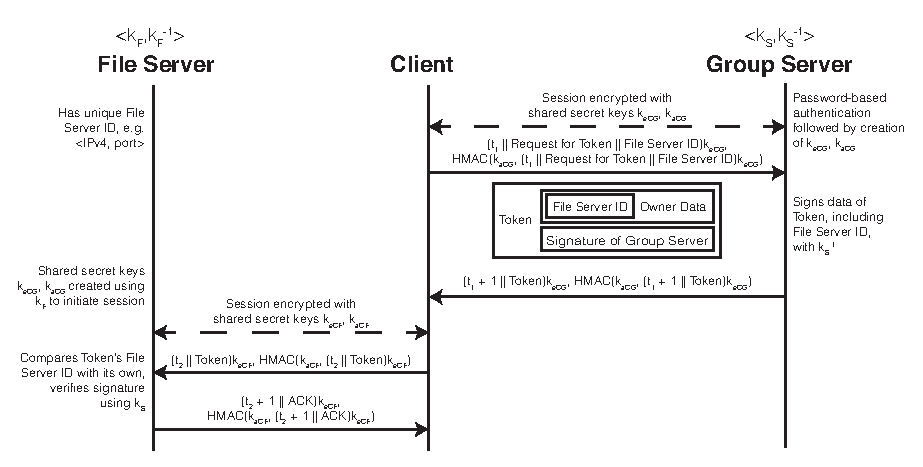
\includegraphics{threat7.eps}
\caption{Threat 7 Mechanism}
\label{threat7}
\end{center}
\end{figure}
\subsection{Correctness and Security of Mechanism}
The correctness of the mechanism lies in the handling of the File Server ID. The user must pass to the Group Server the correct address and port of the File Server to be contacted (e.g., avoid a typo), or else it will be rejected by that File Server. The File Server must also be able to determine its own IP address and port number for comparison to the File Server ID in the token.
	The security of this mechanism is technically only provided by previous mechanisms which would protect the token from attack during transmission. Since the information in the File Server ID can hardly be considered a secret (i.e., the public address and port of a server) then no secret information has been added to the token. However, a case can be made that the Group Server's signature of the token after the File Server ID has been added to it is a protection against modification, which is a security measure.
% Discussion and Commentary
\section{Discussion and Commentary}
Of the three mechanisms created, the mechanism for Threat 5 may be doing the most work of the three. All messages between a client and a server are protected by this mechanism, and thus its importance is equal in magnitude to its frequency of use. Protecting against Threats 6 and 7 is important due to the possibility of malicious File Servers, but without the Threat 5 mechanism there is the possibility of message tampering which could undermine their mechanism's effectiveness. Even if we assumed all clients and servers were 100\% legitimate, messages still have to travel over networks that may be subject to eavesdropping and/or tampering, and thus ensuring the authenticity of each message is paramount to security.

An alternate model for Threat 6 was initially devised. It would have offered file-specific passwords created by the Group Server based on the 3-tuple \{group name, file path, group key version number\}. Compared to the mechanism we presented in this paper, in which the leakage of a single key could result in decryption in any number of leaked files, this other model offered additional security in that the leakage of one single key would only be useful for decrypting one single file. However, it would also have required a heavy increase in network traffic between a File Client and the Group Server, requiring the creation and communication of keys for each upload as well as communication to retrieve a key for a download. Embedding keys in a token would have solved the download issue in the short term, but eventually the number of keys could bloat the token size unnecessarily. It was an interesting idea that may see the daylight again someday.
% Threats 1 through 4 revisited
\section{Threats 1 through 4 revisited}
Not only do our protocols for Threats 5-7 need to protect against their given threats, but they must also not invalidate any of the protocols implemented for Threats 1-4. We will briefly examine the first four threats and show that they remain at least as effective in this Phase 4 as they were in Phase 3.
\subsection{Threat 1: Unauthorized Token Issuance}
None of the mechanisms of Threats 5-7 detract from the effectiveness of our Threat 1 protocol. The Threat 1 protocol is actually enhanced by the Threat 5 mechanism, which prevents the session between the user and the Group Server from modification or replay. The threat of replay is especially important, as a malicious user could replay the challenge/username/password messages and receive another user's token. Additionally, the mechanism for Threat 7, while adding information to the token, does not affect its security.
\subsection{Threat 2: Token Modification/Forgery}
None of the mechanisms of Threats 5-7 detract from the effectiveness of our Threat 2 protocol. Our Threat 7 mechanism adds an additional layer of security above that of Threat 2 in how it requires a token to only be accepted at one particular server. Since the token is signed after that information is embedded in it, modification becomes easily detectable. Furthermore, the transmission of tokens over the network has been made secure from modification via our Threat 5 mechanism.
\subsection{Threat 3: Unauthorized File Servers}
None of the mechanisms of Threats 5-7 detract from the effectiveness of our Threat 3 protocol. If a token is stolen by a malicious File Server and passed to an unauthorized File Server, our Threat 7 mechanism may provide further protection if the unauthorized File Server follows the protocol and checks the File Server ID in the token against its own address and summarily rejects the token.
\subsection{Threat 4: Information Leakage via Passive Monitoring}
None of the mechanisms of Threats 5-7 detract from the effectiveness of our Threat 4 protocol. Since the mechanism of our Threat 5 protocol protects against active attackers, the same level of security applies to passive monitoring as well. Therefore our Threat 5 protocol is an enhancement of the Threat 4 mechanism, which is apt since that is what it was built upon.
\end{document}
